% Copyright (C) 2022 Haoqing Xu
% School of Artificial Intelligence, Southeast University.
% --------------------------------------------------------------------------

% This work may be distributed and/or modified under the
% conditions of the LaTeX Project Public License, either
% version 1.3c of this license or (at your option) any later
% version. This version of this license is in
%    http://www.latex-project.org/lppl/lppl-1-3c.txt
% and the latest version of this license is in
%    http://www.latex-project.org/lppl.txt
% and version 1.3 or later is part of all distributions of
% LaTeX version 2005/12/01 or later.

% This work has the LPPL maintenance status `maintained'.
% The Current Maintainer of this work is Haoqing Xu.

% Home Page of the Project: https://github.com/SuikaXhq/seu-bachelor-thesis-2022
\documentclass{seuthesis-2022}


\title{}
\titlea{}
\titleb{}
\author{}
\studentnum{}
\department{}
\major{}
\supervisor{}
\date{}

\begin{document}

\maketitle

\makedeclaration

\begin{abstract}[zh]
    
\end{abstract}

\begin{abstract}[en]
    
\end{abstract}

\tableofcontents

\section{绪论}
\subsection{课题背景和意义}
绪论部分主要论述选题的意义、国内外研究现状以及本文主要研究的内容、研究思路以及内容安排等。

章标题为三号黑体加粗居中;一级节标题(如,2.1 本文研究内容):四号黑体居左;二级节标题(如,2.1.1 实验方法):小四号宋体居左。

正文部分为小四号宋体,行间距1.5倍行距,首行缩进2个字符。

\subsection{研究现状}

\subsection{本文研究内容}

\subsection{正文}
正文部分每一章应另起页书写书写,层次要清楚,内容要有逻辑性,正文一般不少于15000字。正文部分因学科、选题特点可有差异,但必须言之成理,论据可靠,严格遵循本学科国际通行的学术规范。

中文为小四号宋体,英文及数字为小四号Times New Roman,首行缩进2个字符,行间距为1.5倍。

\subsection{插图格式要求}
插图力求精炼,且每个插图均应有图序和图名。图序与图名位于插图下方,图序一般按章节编排,如图1-1(第一章第1个图),在插图较少时可以全文连续编序,如图10。

如一个插图由两个及以上的分图组成,分图用(a)、(b)、(c)等标出,并标出分图名。

简单文字图可用WORD直接绘制,复杂的图考虑使用相应的图形绘制软件完成,以提高图形表达质量。

插图居中排列,与上文文本之间空一行。图序图名设置为五号宋体居中,图序与图名之间空一格。

\begin{figure}[H]
    \centering
    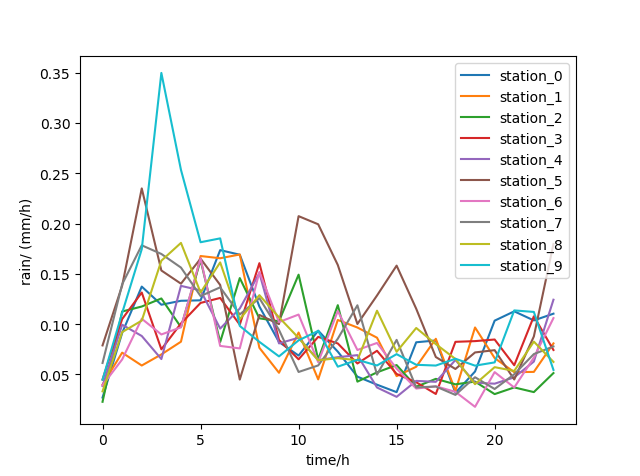
\includegraphics{fig/降水量均值分布图.png}
    \caption{每小时降水量24小时均值分布图}
    \label{fig:1}
\end{figure}

\begin{figure}[H]
    \centering
    \subcaptionbox{速度障碍集合\label{fig:2a}}
      {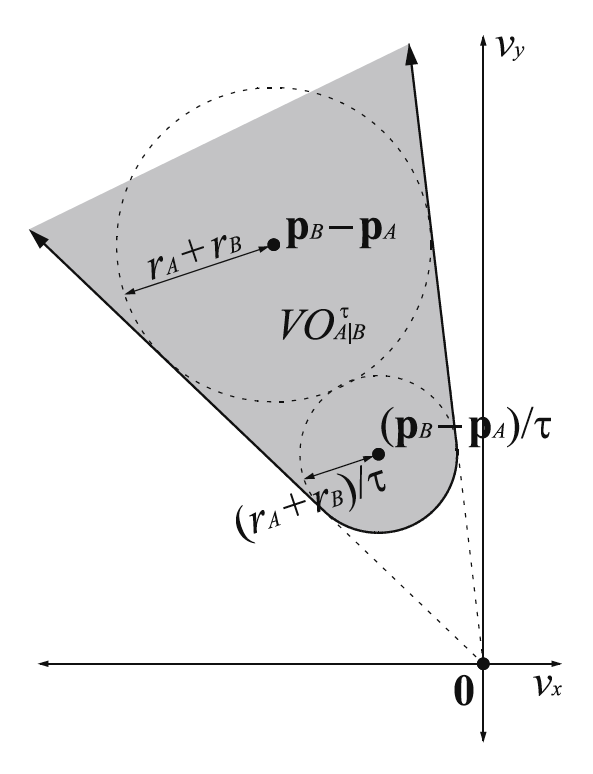
\includegraphics{fig/速度障碍集合.png}}
    \subcaptionbox{速度障碍集合\label{fig:2b}}
      {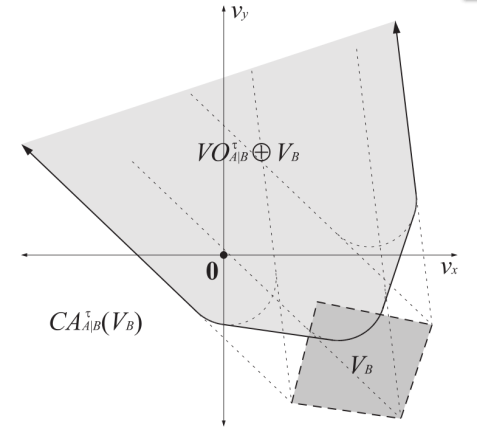
\includegraphics{fig/避免碰撞集合.png}}
    \caption{速度障碍法速度选择}
    \label{fig:2}
\end{figure}

\subsection{表格格式要求}
表格的结构应简洁,一律采用三线表,应有表序和表名,且表序和表名位于表格上方。表格可以逐章单独编序(如:表2.1),也可以统一编序(如:表10),采用哪种方式应和插图及公式的编序方式统一。表序必须连续,不得重复或跳跃。

表格无法在同一页排版时,可以用续表的形式另页书写,续表需在表格右上角表序前加“续”字,如“续表2.1”,并重复表头。

表格居中,边框为黑色直线1磅,中文为五号宋体,英文及数字为五号Times New Roman字体,表序与表名之间空一格,表格与下文之间空一行。

\subsection{表达式}
论文中的公式应注序号并加圆括号,序号一律用阿拉伯数字连续编序(如(28))或逐章编序(如(3.6)),编号方式应与插图、表格方式一致。序号排在版面右侧,且距右边距离相等。公式与序号之间不加虚线。

长公式在一行无法写完的情况下,原则上应在等号(或数学符号,如“+”、“-”号)处换行,数学符号在换行的行首。

公式及文字中的一般变量(或一般函数)(如坐标X、Y,电压V,频率f)宜用斜体,矢量用粗斜体如S或白斜体上加单箭头,常用函数(如三角函数cos、对数函数ln等)、数字运算符、化学元素符号及分子式、单位符号、产品代号、人名地名的外文字母等用正体。

公式排版时可选中模板中的“公式式样”,先将光标移至公式前,按“Tab”键,公式居中;再将光标移至编号前,按“Tab”键移动一个制表符位置,使公式编号右对齐。

\subsection{注释}

正文中有个别名词或情况需要解释时,可加注说明,注释采用页末注(将注文放在加注页的下端)。在引文的右上角标注序号①、②、……,如“马尔可夫链 ”。若在同一页中有两个以上的注时,按各注出现的先后,顺序编号。引文序号,以页为单位,且注释只限于写在注释符号出现的同页,不得隔页。

注释采用小五号宋体,英文及数字为小五号Times New Roman字体,利用“引用”插入脚注功能插入。

\chapter{总结与展望}
\bibliographystyle{gbt7714-numerical}
\bibliography{reference.bib}
\end{document}